\input{Dissertation/appendixsetup}   % Предварительные настройки для правильного подключения Приложений

\chapter{Общие сведения о плазме и УТС} \label{Appendix0}

\section{Общие сведения о плазме}

В любом газе некоторое количество атом ионизовано. Таким образом, в газе помимо нейтральных атомов с концентрацией $n_n$ содержатся и некоторое количество ионов и электронов, концентрации которых соответственно обозначают как $n_i$ и $n_e$. Ионы обычно только однократно ионизированы, т. е.
\begin{equation}
n_e \approx n_i^I.
\end{equation}
Вводится очень важный параметр --- степень ионизации газа. Он, очевидно, выражается как
\begin{equation}
k_c = \frac{n_e}{n_n}.
\end{equation}

При достаточно больших концентрациях и степени ионизации взаимодействие положительно и отрицательно заряженных частиц приводит к поддержанию макроскопической нейтральности в объемах, сравнимых по размеру с объемом газа; при этом нарушения макроскопической нейтральности приводят к появлению сильных электрических полей, быстро восстанавливающих ее. Ионизованный газ при таких концентрациях и называется \textit{плазмой}. Это название было предложено в 1923 г. И. Ленгмюром при изучении электрических разрядов в лампах заполненных ионизированным газом \cite{golant,kotelnikov2008}.


Плазма является самым распространенным известным на сегодняшний день состоянием вещества, в силу того, что все звезды, атмосферы планет и межзвездный газ по большей части находятся именно в состоянии плазмы. Помимо этого плазма --- это естественное состояние сильно разогретого вещества \cite{golant,archenovich}.

Температуру в физике плазмы принято изменять в энергетических единицах, а именно
\begin{equation}
\left[T\right] = \left[\text{эВ}\right].
\end{equation}
Везде далее под температурой будет иметься в виду именно энергетическая температура, если не указано иначе. Её связь с абсолютной температурой $T_K$ даётся выражением
\begin{equation}
T = k T_K,
\end{equation}
где $k$ --- постоянная Больцмана. Связь средней энергии теплового движения частиц $W$ с температурой плазмы, как и для любого равновесного газа с тремя степенями свободы, дается равенством
\begin{equation}
W = \frac{3}{2} T.
\end{equation}

Очень часто плазма является неравновесной. Для того, чтобы корректно описывать её поведение в подобных случая вводят две температуры: ионная температура $T_i$ и электронная температура $T_e$.

Как уже упоминалось выше, любое нарушение микроскопической нейтральности приводит к появления сильных полей, которые стремятся всё уравновесить. Однако, существует некоторый предельный объём, квазинейтральность внутри которого может быть свободно нарушена благодаря тепловому движению частиц плазмы. Простейшая оценка характерного расстояния при котором это происходит даёт следующее выражение:
\begin{equation}
r_D = \sqrt{\frac{T_e \varepsilon_0}{n_e e^2}},
\end{equation}
где $e$ --- элементарный заряд. Это величину называют \textit{радиусом Дебая}.

\section{Управляемый термоядерный синтез}

\subsection{Основные реакции}

Известна \cite{sivuhin5} экспериментальная зависимость удельной энергии связи $E_{\text{св}}/A$ ядра от количества нуклонов $A$ в этом ядре (рисунок \ref{fig:link_energy}).  Из анализа данной зависимости можно сделать вывод о существовании двух различных типов энергетически выгодных ядерных реакций: соединение (синтез) легких ядер и распад тяжелых ядер. Человечество хорошо освоило второй способ, доказательством тому служит существование множества АЭС. Однако, существует главная проблема --- недостаток сырья, тяжёлые элементы редки.

Синтез легких элементов имеет два основных преимущества: практически нескончаемые запасы топлива и более энергетически выгодная реакция. К минусам же относятся огромные технологические и инженерные проблемы при попытки его осуществления \cite{lukyanov}.

Проводить реакцию используя систему пушка-мишень не представлялось возможным, т. к. сечение реакции слишком мало. Лишь одна из многих тысяч ускоренных  частиц, падающих на мишень, вызывает ядерную реакцию. Остальные непроизводительно расходуют запасённую энергию малыми порциями на ионизацию и возбуждение атомов.

\begin{figure}[h]
\centering
\includegraphics[width=0.7\linewidth]{../fig/ch1/link_energy}
\caption{Зависимость удельной энергии связи ядра от числа нуклонов в этом ядре}
\label{fig:link_energy}
\end{figure}

Тогда в 1950 г. И. Е. Таммом и А. Д. Сахоровым было предложено использовать следующую схему, в которой газ из необходимых элементов доводят до состояния плазмы со средней тепловой энергией движения достаточной для термоядерной реакции ( $W \sim 10 \div 100$ кэВ, энергия достаточная для преодоления кулоновского барьера). Далее, удержание полученной системы было предложено некой сложной \textit{магнитной ловушкой}.


Практический интерес представляют две известные реакции\cite{dnestrovsky}:
\begin{enumerate}
\item $D,D$-реакция. Может идти равновероятно одним из двух способов:
\begin{equation}
D + D \to
\begin{cases}
\left( ^3He + 0,82 \text{ МэВ}  \right) + \left( n + 2,45 \text{ МэВ} \right) \\
\left( T + 1,01 \text{ МэВ}  \right) + \left( p + 3,03 \text{ МэВ} \right)
\end{cases}.
\end{equation}
\item $D,T$-реакция:
\begin{equation}
D + T \to \left( ^4He + 3,52 \text{ МэВ}  \right) + \left( n + 14,06 \text{ МэВ} \right)
\label{eq:DT_rec}
\end{equation}.
\end{enumerate}

$D,T$-реакция сопровождается более интенсивным выделением энергии, а её сечение  в 50-100 раз превышает обе $D,D$-реакции, поэтому она более предпочтительна.

Стоит отметить, что значительную часть энергии получает нейтрон --- нейтральная частица. Отсутствие у неё заряда ставит большую проблему о том, как использоваться эту энергию, ведь электромагнитные поля здесь уже бессильны.

\subsection{Критерий Лоусона}

Необходимо прикладывать огромное количество энергии для того, чтобы удерживать горячую плазму достаточного объема и плотности. В 1957 году британским физиком Дж. Д. Лоусоном  был предложен оценочный критерий о положительном выходе термоядерной реакции \cite{Lawson}. Его рассуждения основывались на простом неравенстве
\begin{equation}
W_{\text{яд}} - W_{\text{тор}} - W_{\text{ост}} > 0, 
\end{equation}
где $W_{\text{яд}}$ --- энергия термоядерной реакции, $W_{\text{тор}}$ --- потери на тормозное излучение,  $W_{\text{ост}}$ --- остальные потери, которые некоторым пропорциональны $nT$. В своих рассуждениях Лоусон приходит к следующему неравенству:
\begin{equation}
n \tau > f(T) = \frac{T}{C_1 E_{\text{р}} <\sigma u> - C_2 \sqrt{T}},
\label{eq:Lowson_cr}
\end{equation}
где $E_{\text{р}}$ --- энергетический выход реакции, $u$ --- относительная скорость реагирующих ионов, $\sigma$ --- сечение реакции, $\tau$ --- характерное время удержания, $n$ --- концентрация ионов, $C_1,C_2$ --- некоторые константы. 

Функция $f(T)$ в правой части неравенства \eqref{eq:Lowson_cr} имеет минимум, так как при малых $T$ быстро уменьшается $<\sigma u>$, а при больших $T$ растёт числитель. Для $D,T$-реакции минимум функции находится \cite{kotelnikov} при $T_{\min} \approx 23 \text{ кэВ}$ (рисунок \ref{fig:f_T_Lowson}). 

\begin{figure}
\centering
\includegraphics[width=0.5\linewidth]{./fig/ch1/f_T_Lowson}
\caption{График зависимости функции $f(T)$ для $D,T$-реакции}
\label{fig:f_T_Lowson}
\end{figure}


Одним из основных параметров любой ловушки является \textit{параметр удержания} $n \tau$.


\subsection{Некоторые характерные параметры плазменных ловушек}

В случае создания термоядерного синтеза, кроме критерия Лоусона \eqref{eq:Lowson_cr}, выделяют параметр $Q$, равный отношению выделяемой мощности реактора, к его потребляемой мощности. Таким образом, глобально ставится задача создания реактора с $Q>1$.

Также очень важным параметром является параметр $\beta$. Это есть отношение плазменного давления, к магнитному давлению в ловушке:
\begin{equation}
\beta = \frac{P_{plasma}}{P_{mag}} = \frac{nT}{B^2/2 \mu_0}.
\end{equation}

Для токамаков (установок с закрытой конфигурацией магнитного поля и торообразными магнитными поверхностями) выделяют ещё один параметр $q$ --- \textit{величина запаса устойчивости}. $q$ численно равняется отношению числа обходов $m$ по большому радиусу тора к числу $n$ обходов по малому радиусу тора. Если $q = m/n$ является простой дробью, то данный случай соответствует резонансной поверхности. А так как в сильном магнитном поле частицы дрейфуют вдоль магнитных силовых линий, то этот случай означает \textit{вырожденность магнитной линии}, от этого всегда стараются избавляться, т. к. это приводит к неустойчивости. 


\chapter{Численное решения уравнения движения} \label{AppendixA}


\section{Численное решение уравнения движения}

Поставим задачу представить уравнение движения релятивистской частицы в удобном для численного расчёта виде. Запишем уравнение движения в общем виде
\begin{equation}
\frac{d \vec{p}}{dt} = \vec{F},
\label{eq:Newton_for_numeric}
\end{equation}
где $\vec{p}$ --- импульс частицы, а $\vec{F}$ --- сила действующая на частицу. 

Есть несколько подходов к разрешения данной задачи.

\subsection{Численное решение уравнения движения через импульс частицы}


Известны релятивистские соотношения для полной энергии $\mathscr{E}$ и для импульса:
\begin{eqnarray*}
	\mathscr{E} &=& \frac{mc^2}{\sqrt{1 - v^2/c^2}},\\ \nonumber \\
	\vec{p} &=& \frac{m\vec{v}}{\sqrt{1 - v^2/c^2}}.
\end{eqnarray*}
Отсюда следует, что
\begin{equation}
	\vec{v} = \frac{\vec{p}c^2}{\mathscr{E}}.
\end{equation}
С другой стороны, известно, что $\mathscr{E} = \sqrt{p^2c^2 + m^2 c^4}$.
Принимая во внимания определение скорости, запишем
\begin{equation}
	\frac{d\vec{r}}{dt} = \frac{c \vec{p}}{\sqrt{p^2 + m^2 c^2}}.
	\label{eq:drdt_rel}
\end{equation}
Тогда из \eqref{eq:Newton_for_numeric} и \eqref{eq:drdt_rel} несложно получить систему из шести дифференциальных уравнения первого порядка:
\begin{equation}
	\begin{cases}
	\dot{p}_x = F_x, \qquad \dot{p}_y = F_y, \qquad \dot{p}_z = F_z, \\ \\
	\dot{x} = \dfrac{c p_x}{\sqrt{p^2 + m^2 c^2}}, \\ \\
	\dot{y} = \dfrac{c p_y}{\sqrt{p^2 + m^2 c^2}}, \\ \\
	\dot{z} = \dfrac{c p_z}{\sqrt{p^2 + m^2 c^2}}.
	\end{cases}
	\label{eq:style1}
\end{equation}

\subsection{Численное решение уравнения движения через ускорение частицы}

Расписав полную производную по времени в \eqref{eq:Newton_for_numeric}, имеем
\begin{equation}
\beta \frac{d \vec{v}}{dt} + \frac{\beta^3}{c^2} (\vec{v} \cdot \frac{d \vec{v}}{dt}) \vec{v} = \vec{f},
\end{equation}
где $\vec{f} = \vec{F}/m$ --- приведённая сила. Перейдя к компонетной записи, запишем
\begin{eqnarray*}
\begin{cases}
\dot{v}_x \beta \left(1 + \frac{\beta^2}{c^2} v_x^2 \right) +
\dot{v}_y \frac{\beta^3}{c^2} v_x v_y + 
\dot{v}_z \frac{\beta^3}{c^2} v_x v_z  = f_x, \\

\dot{v}_x \frac{\beta^3}{c^2} v_x v_y +
\dot{v}_y \beta \left(1 + \frac{\beta^2}{c^2} v_y^2 \right) + 
\dot{v}_z \frac{\beta^3}{c^2} v_y v_z  = f_y, \\

\dot{v}_x  \frac{\beta^3}{c^2} v_x v_z +
\dot{v}_y \frac{\beta^3}{c^2} v_y v_z + 
\dot{v}_z \beta \left(1 + \frac{\beta^2}{c^2} v_z^2 \right)  = f_x.
\end{cases}
\end{eqnarray*}

Решим данную систему методом Крамера относительно $\dot{v}_x$, $\dot{v}_y$ и $\dot{v}_z$. 
Главный определитель:
\begin{equation*}
\Delta = \beta^3 + \beta^5 \frac{v^2}{c^2} \neq 0.
\end{equation*}
Побочные определители:
\begin{eqnarray*}
\Delta_x &=& f_x \beta^2 \left( 1+ \frac{\beta^2}{c^2} (v^2_y +  v_z^2) \right)  - f_y \frac{\beta^4}{c^2} v_x v_y - f_z \frac{\beta^4}{c^2} v_x v_z, \\ \\
\Delta_y &=& -f_x \frac{\beta^4}{c^2} v_x v_y + f_y \beta^2 \left( 1 + \frac{\beta^2}{c^2}(v_x^2 + v_z^2) \right)  - f_z \frac{\beta^4}{c^2} v_y v_z, \\ \\
\Delta_z &=& - f_x \frac{\beta^4}{c^2} v_x v_z - f_y \frac{\beta^4}{c^2} v_y v_z + f_z \beta^2 \left( 1 + \frac{\beta^2}{c^2} (v_x^2 +  v_y^2) \right).
\end{eqnarray*}
Тогда решение запишется в виде \cite{iliin_algebra}
\begin{equation*}
\dot{v}_x = \frac{\Delta_x}{\Delta}, \qquad \dot{v}_y = \frac{\Delta_y}{\Delta}, \qquad \dot{v}_z = \frac{\Delta_z}{\Delta}.
\end{equation*}
То есть
\begin{equation*}
\begin{cases}
\dot{v}_x = \dfrac{f_x (1+ \frac{\beta^2}{c^2}  [ v^2_y +  v_z^2 ]) - \frac{\beta^2}{c^2} ( f_y v_x v_y + f_z v_x v_z) }{\beta \left( 1 + \frac{\beta^2 v^2}{c^2}\right) }, \\ \\

\dot{v}_y = \dfrac{-f_x \frac{\beta^2}{c^2} v_x v_y + f_y (1 + \frac{\beta^2}{c^2} [v_x^2 + v_z^2]) - f_z \frac{\beta^2}{c^2} v_y v_z }{\beta \left( 1 + \frac{\beta^2 v^2}{c^2} \right) }, \\ \\

\dot{v}_z = \dfrac{- f_x \frac{\beta^2}{c^2} v_x v_z - f_y \frac{\beta^2}{c^2} v_y v_z + f_z (1 + \frac{\beta^2}{c^2} [v_x^2 + 2 v_y^2]) }{\beta \left( 1 + \frac{\beta^2 v^2}{c^2}\right) }. 
\end{cases}
\end{equation*}
Преобразовав, получим систему из шести дифференциальных уравнения первого порядка:

\begin{equation}
\begin{cases}
\dot{v}_x = \dfrac{f_x  + \frac{\beta^2}{c^2} \left[ f_x \left(v_y^2 + v_z^2\right) - f_y v_x v_y  - f_z v_x v_z  \right] }{\beta^3 }, \\ \\

\dot{v}_x = \dfrac{f_y  + \frac{\beta^2}{c^2} \left[ f_y \left(v_x^2 + v_z^2\right) - f_x v_x v_y  - f_z v_y v_z  \right] }{\beta^3}, \\ \\

\dot{v}_x = \dfrac{f_z  + \frac{\beta^2}{c^2} \left[ f_z \left(v_x^2 + v_y^2\right) - f_x v_x v_z  - f_y v_y v_z  \right] }{\beta^3}, \\ \\

\dot{x} = v_x, \qquad \dot{y} = v_y, \qquad \dot{z} = v_z.
\end{cases}
\label{eq:style2}
\end{equation}
Стоит напомнить, что
\begin{equation*}
\beta = \frac{1}{\sqrt{1 - v^2/c^2}} = \frac{1}{\sqrt{1 - \frac{v_x^2 + v_y^2 + v_z^2}{c^2}}}.
\end{equation*}


\subsection{Выбор метод решения системы ДУ, метод Рунге-Кутты}

В качестве метода решения системы дифференциальных уравнений (ДУ) был выбран метод Рунге-Кутты 4-го порядка. Данный метод сочетает в себе как довольно небольшое количество математических операций за один шаг, так и очень высокую сходимость\cite{butcher1987numerical}.

Суть метода заключается в следующем. Пусть имеется система ДУ:
\begin{equation*}
	\begin{cases}
		\dot{y}_1 = g_1 (t,y_1,y_2,\dots,y_n), \\
		\dot{y}_2 = g_2 (t,y_1,y_2,\dots,y_n), \\
		\vdots \\
		\dot{y}_n = g_n (t,y_1,y_2,\dots,y_n), 
	\end{cases}
	\qquad 
	\begin{cases}
		y_1 (t_0) = y_{01}, \\
		y_2 (t_0) = y_{02}, \\
		\vdots \\
		y_n (t_0) = y_{0n} 
	\end{cases}
\end{equation*}
или
\begin{equation*}
\dot{\vec{y}} = \vec{g} \left(t , \vec{y}\right), \qquad \vec{y}(0) = \vec{y}_0.
\end{equation*}
Тогда приближенное значение в последующих точках вычисляется по итерационной формуле:
\begin{equation}
\vec{y}_{n+1} = \vec{y}_n + \frac{1}{6} \left( \vec{k}_1 + 2 \vec{k}_2 + 2 \vec{k}_3 + \vec{k}_4  \right),
\end{equation}
где 
\begin{eqnarray}
\vec{k}_1 &=& \vec{g}(t_n,\vec{y}_n) dt, \nonumber \\ \nonumber \\
\vec{k}_2 &=& \vec{g}(t_n + \dfrac{dt}{2},\vec{y}_n + \dfrac{1}{2} \vec{k}_1 ) dt, \nonumber \\  \\
\vec{k}_3 &=& \vec{g}(t_n + \dfrac{dt}{2},\vec{y}_n + \dfrac{1}{2} \vec{k}_2 ) dt, \nonumber \\ \nonumber \\
\vec{k}_4 &=& \vec{g}(t_n + dt,\vec{y}_n + \vec{k}_3) dt, \nonumber
\end{eqnarray}
а $dt$ --- шаг по времени.

Этот метод имеет четвёртый порядок точности, то есть суммарная ошибка на конечном интервале интегрирования имеет порядок $\mathscr{O}(d t^4)$.


\chapter{Алгоритм программы для вычисления эволюции ансамбля заряженных частиц} \label{AppendixB}

Основная идея вычислительной программы заключается в следующем. При каждом запуске в первую очередь идёт загрузка входных данных (параметры пространственной и временной дискретизации, информация о внешних электромагнитных полях, параметры частиц, такие как плотность и температура, и~др.). Далее происходит инициализация (задание начальных координат и скоростей) первоначальных частиц в системе. После этого уже начинается выполнение основного цикла по времени, в котором уже происходит расчёт поля пространственного заряда и решение уравнений движения для всех заряженных частиц (рисунок \ref{fig:Diagram1}). 

\begin{figure}[h!]
\centering
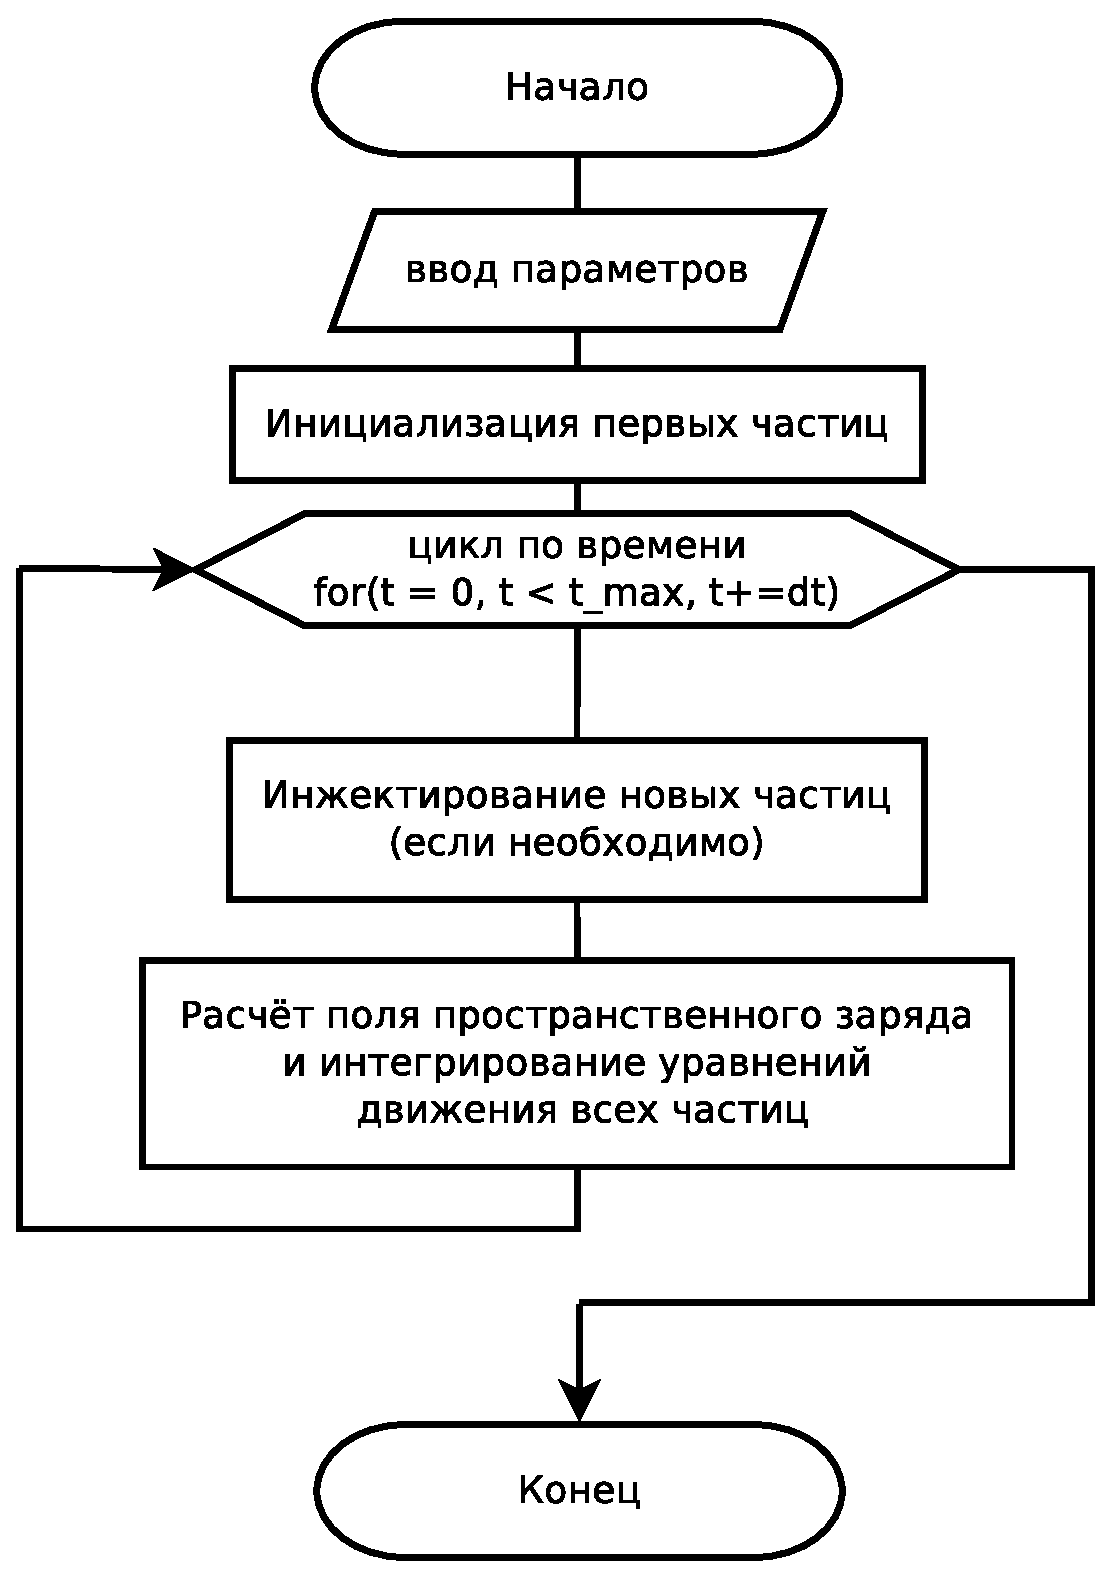
\includegraphics[width=0.5\linewidth]{./fig/ch3/Diagram1}
\caption{Упрощенный базовый алгоритм вычислительной программы}
\label{fig:Diagram1}
\end{figure}

Алгоритм вычислительной программы может значительно различаться в зависимости от того, каким образом рассчитывается поле пространственного заряда. 

В самом общем случае это выражения для полей, полученные из потенциалов Лиенара-Вихерта \cite{Landau2}:
\begin{equation}
	\vec{E} = \dfrac{q}{4 \pi \varepsilon_0} \dfrac{\left( 1 - \dfrac{v^2}{c^2} \right) \left( \vec{R} - \dfrac{\vec{v} R}{c}  \right) }{\left( R - \dfrac{\vec{v} \cdot \vec{ R}}{c} \right)^3} + \dfrac{q}{4 \pi \varepsilon_0 c^2} \dfrac{\left[ \vec{R} , \left[ \vec{R} - \dfrac{\vec{v}R}{c} , \dot{\vec{v}}  \right]  \right]}{\left( R - \dfrac{\vec{v} \cdot \vec{ R}}{c} \right)^3},
	\label{eq:opt_LV_E_early}
\end{equation}
\begin{equation}
	\vec{B} = \frac{1}{c} \frac{\vecmult{R}{E}}{R}.
	\label{eq:opt_LV_B_early}
\end{equation}
Здесь $\vec{R}$ --- радиус вектор, направленный от частицы с зарядом $q$ до точки, в которой рассчитывается поле;  $\dot{\vec{v}} = \partial \vec{v} / \partial \tau$. Все величины в правых сторонах берутся в момент времени $\tau$, определяемым уравнением 
\begin{equation}
	\tau = t - \frac{R(\tau)}{c}.
	\label{eq:wait_for_me}
\end{equation}


Выражения \eqref{eq:opt_LV_E_early} и \eqref{eq:opt_LV_B_early} были получены не используя никакие пренебрежения и упрощения (за исключением представления частицы точечной). В остальном же они учитывают все возможные эффекты, в том числе и излучение при $\dot{\vec{v}} \neq 0$. Однако, плата за такую полноту описания является огромная вычислительная сложность решения. Рассмотрим возможные упрощения и предельные переходы, которые можно сделать.

Первое возможное предположение --- это пренебрежение временем запаздывания, то есть от него ничего не должно зависеть. Отсюда следует, что $\partial \vec{v}/\partial \tau \to 0$.
тогда выражения \eqref{eq:opt_LV_E_early}, \eqref{eq:opt_LV_B_early} редуцируются в следующие:
\begin{eqnarray}
	\vec{E} &=& \dfrac{q}{4 \pi \varepsilon_0} \dfrac{\left( 1 - \dfrac{v^2}{c^2} \right) \left( \vec{R} - \dfrac{\vec{v} R}{c}  \right) }{\left( R - \dfrac{\vec{v} \cdot \vec{ R}}{c} \right)^3} , \\ \nonumber \\
	\label{eq:opt_LV_E_easy}
	\vec{B} &=& \dfrac{1}{c} \frac{\vecmult{R}{E}}{R}.
	\label{eq:opt_LV_B_easy}
\end{eqnarray}

Следующим шагом в упрощении может стать дорелятивизм. Иначе говоря, если
$v/c \to 0$,
то выражения для полей примут наиболее простой вид
\begin{eqnarray}
\vec{E} &=& \dfrac{q}{4 \pi \varepsilon_0}  \dfrac{ \vec{R} }{R^3}, \label{eq:opt_LV_E_easiest} \\ \nonumber \\
\vec{B} &=& 0.
\label{eq:opt_LV_B_easiest}
\end{eqnarray}


Рассмотрим два предельных случая --- согласно уравнениям \eqref{eq:opt_LV_E_early} и \eqref{eq:opt_LV_B_early}, которые учитывают времена запаздывания, и согласно уравнениям \eqref{eq:opt_LV_E_easiest} и \eqref{eq:opt_LV_B_easiest}.

\section{Релятивистское движение с учётом запаздывание}

Рассмотрим численный алгоритм расчёта полей согласно уравнениям, полученным из потенциалов Лиенара-Вихерта. Основная сложность заключается в решении уравнения \eqref{eq:wait_for_me} для определения времени запаздывания $\tau$.

\begin{figure}[h!]
\centering
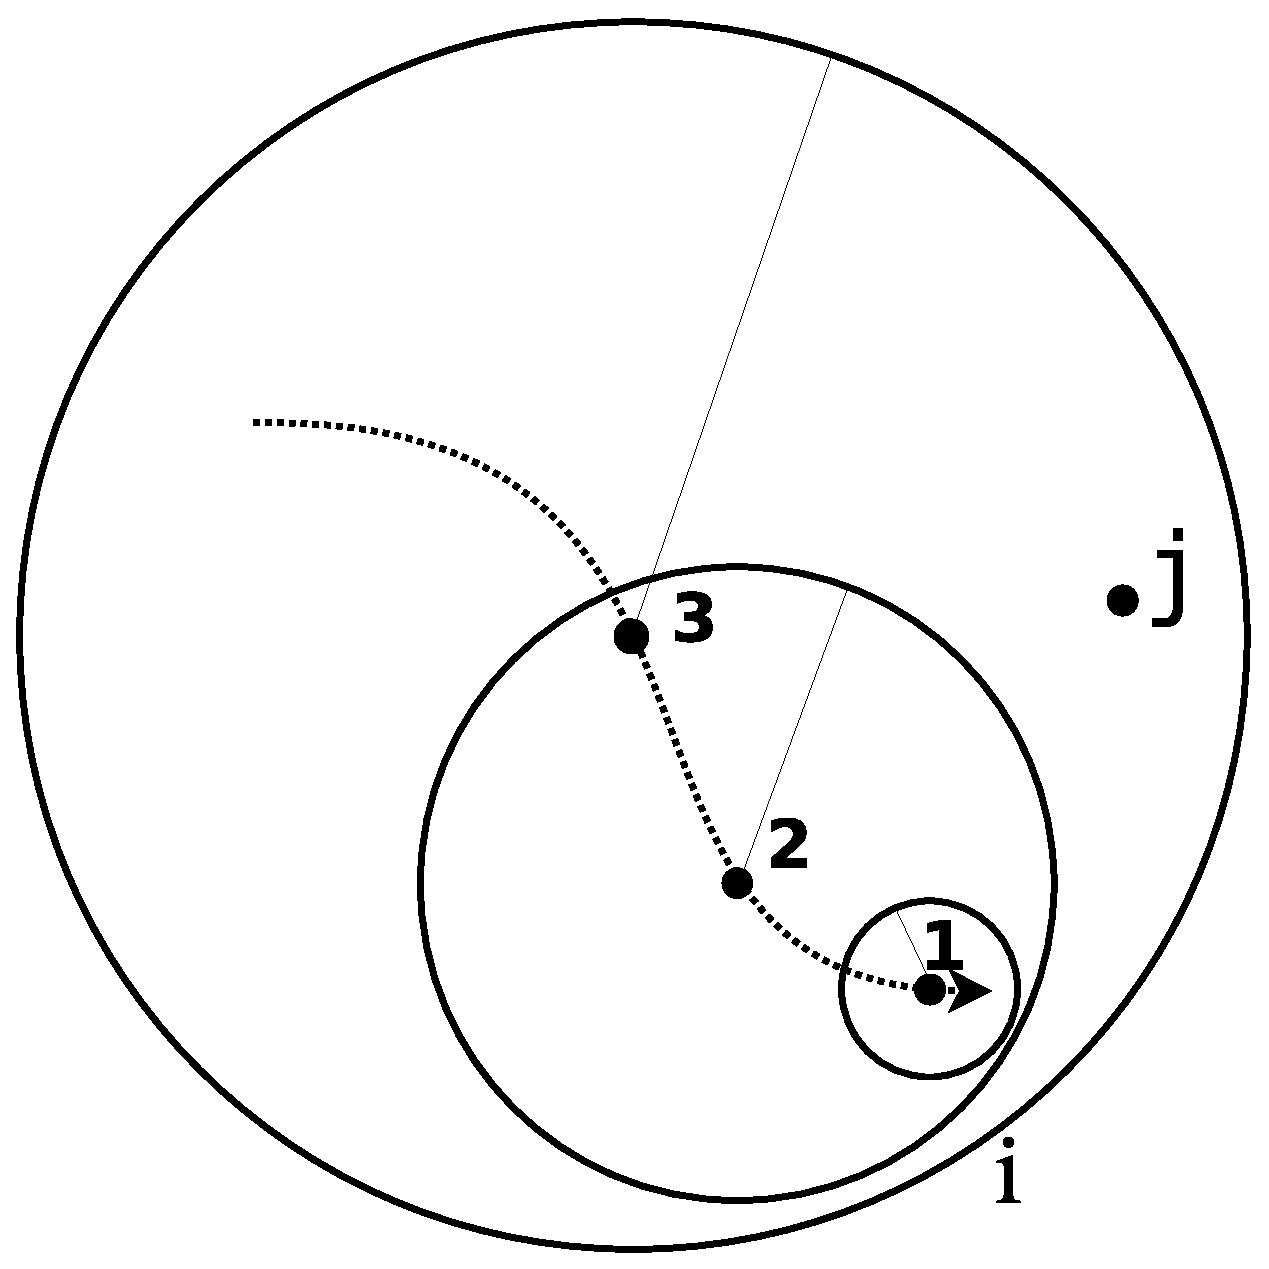
\includegraphics[width=0.5\linewidth]{./fig/ch3/Diagram2tau}
\caption{Графическое представление решения уравнения \eqref{eq:wait_for_me}}
\label{fig:Diagram2tau}
\end{figure}

Решить его можно следующим образом. Пусть есть траектория $i$-й частицы и необходимо найти то время, за которое сигнал от этой самой $i$-й частицы дошел до некоторой $j$-й частицы. Сигнал распространяется в вакууме, как известно, со скоростью $c$, значит необходимо построить сферу взаимодействия для каждого шага, радиус которой будет равен $k \cdot cdt$, $k$ --- количество шагов <<в прошлое>> (рисунок \ref{fig:Diagram2tau}). Строить данные сферы необходимо до тех пор, пока расстояние до $j$-й частицы не станет меньше радиуса сферы
\begin{equation}
r_{ij} \leqslant k' c dt,
\end{equation}
тогда
\begin{equation}
\tau = k' dt.
\end{equation}
Далее, алгоритм действий внутри цикла по времени представлен на рисунке \ref{fig:Diagram3}.

\begin{figure}[h!]
\centering
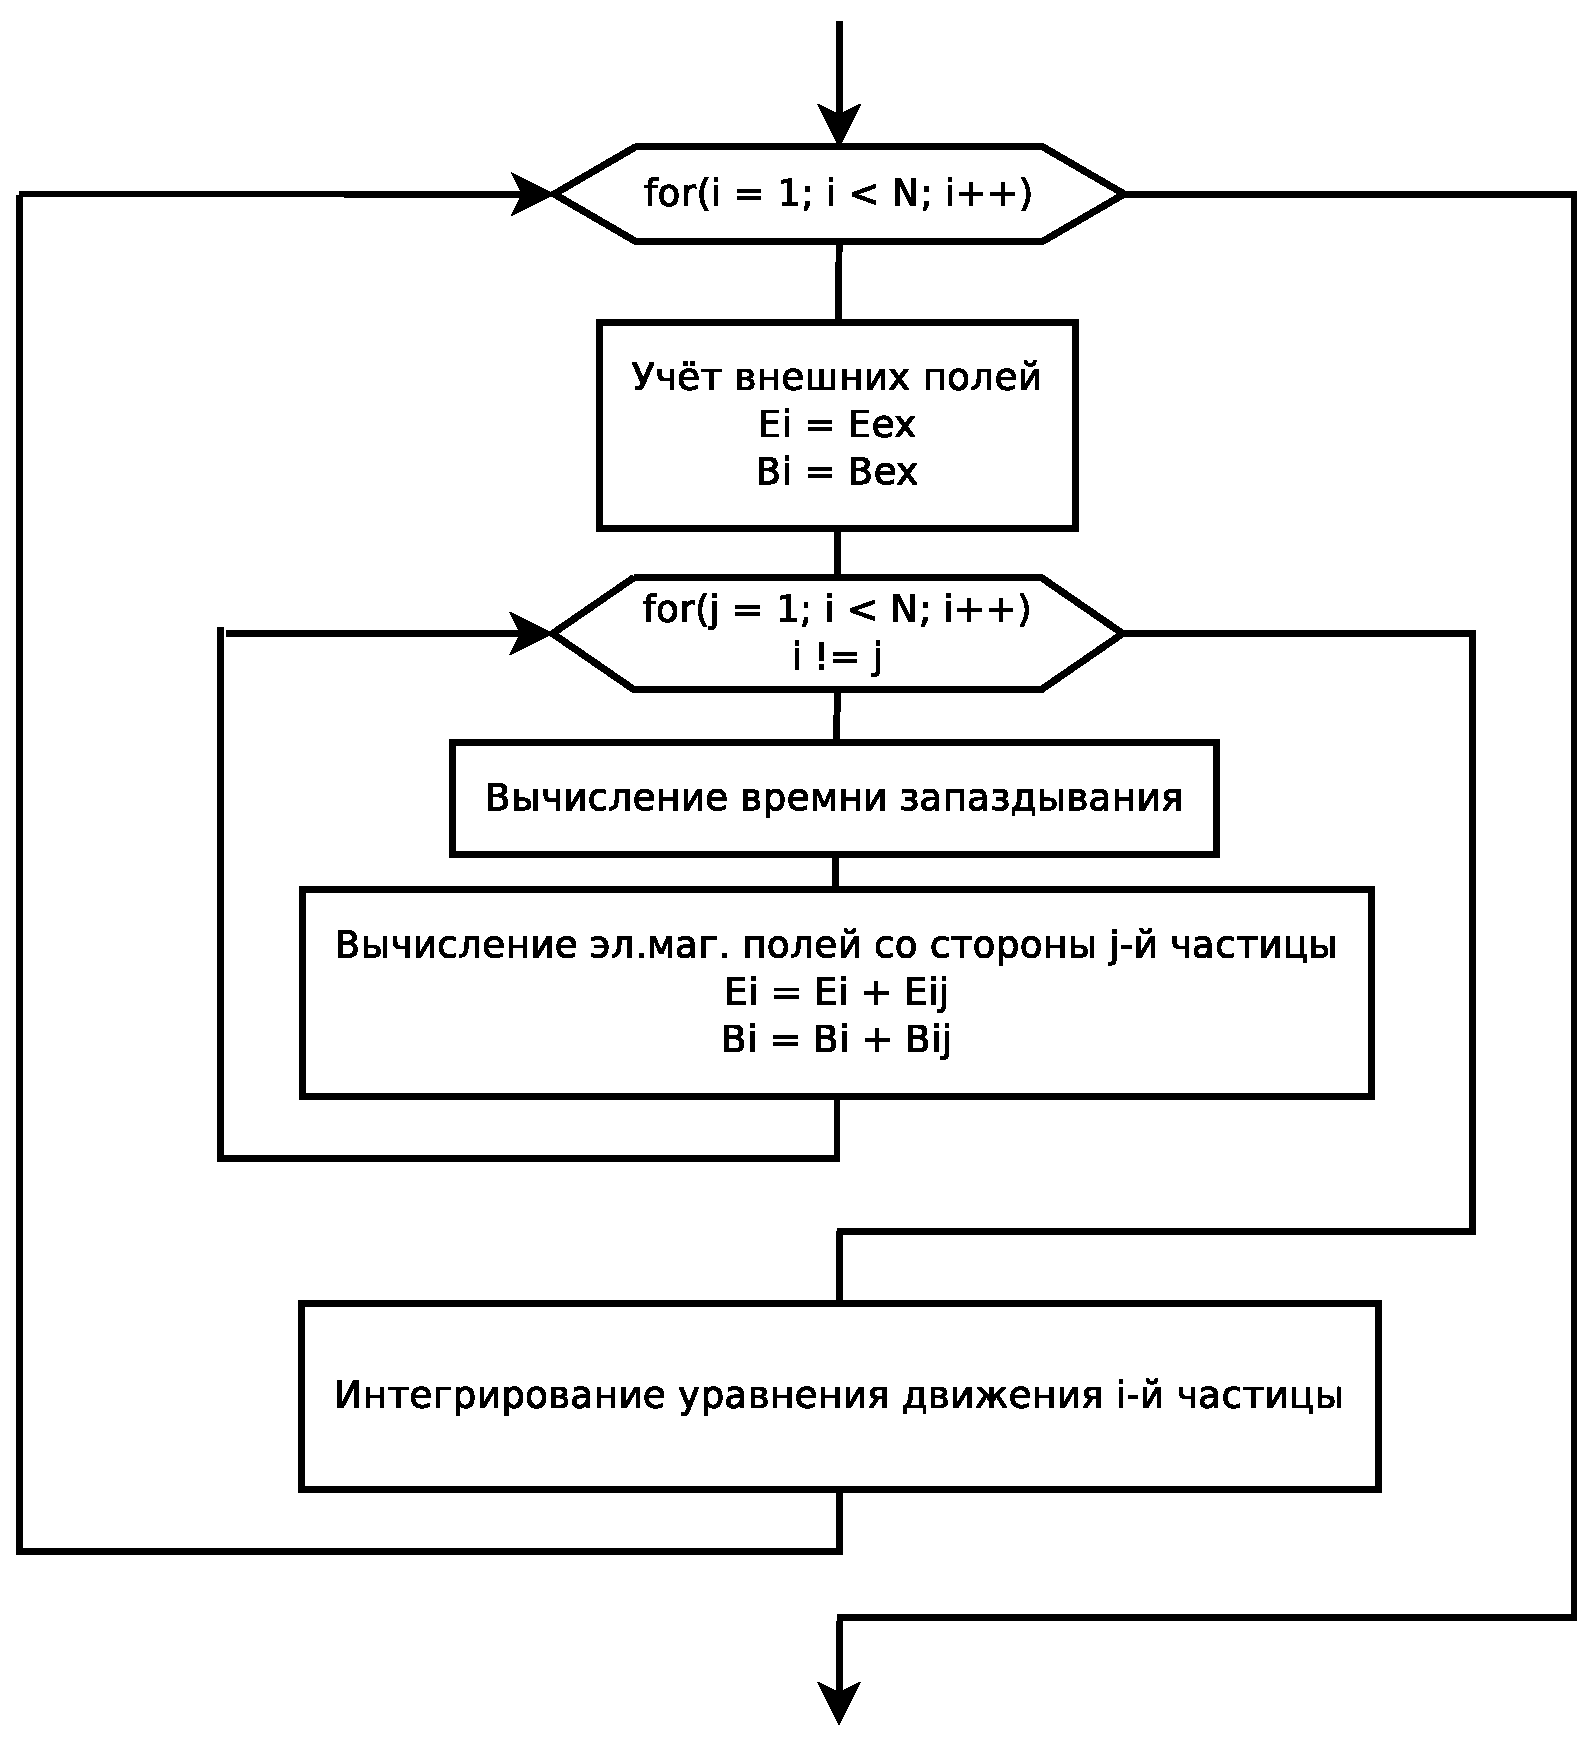
\includegraphics[width=0.7\linewidth]{./fig/ch3/Diagram3}
\caption{Алгоритм действий внутри цикла по времени с учётом потенциалов запаздывания}
\label{fig:Diagram3}
\end{figure}


\section{Нерелятивистское движение без учёта запаздывания}

В другом предельном случае, когда $R/c$ пренебрежительно мало и $v/c \to 0$, можно значительно ускорить процесс вычислений, если воспользоваться напрямую третьим законом Ньютона:
\begin{equation}
\vec{F}_{ij} = - \vec{F}_{ji},
\end{equation}
где $\vec{F}_{ij}$ --- сила взаимодействия $i$-й частицы на $j$-ю частицу, а $\vec{F}_{ji}$ --- наоборот.  В случае кулоновского потенциала при дебаевской экранировке сила взаимодействия будет вычисляться следующим образом:
\begin{equation*}
	\vec{F}_{ij} = - \nabla \left[U_{ij} (r_{ij}) \cdot \Phi \left( \frac{r_{ij}}{r_D} \right)\right] = - \nabla \left[ \frac{1}{4 \pi \varepsilon_0} \frac{q_i q_j}{r_{ij}} \cdot e^{r_{ij}/r_D} \right],
\end{equation*}
\begin{equation}
	\vec{F}_{ij} = 
	\begin{cases}
		\dfrac{1}{4 \pi \varepsilon_0} \dfrac{q_iq_j \left( \vec{r}_i - \vec{r}_j \right)}{r_{ij}^2} e^{-r_{ij}/r_D} \left( \dfrac{1}{r_{ij}} - \dfrac{1}{r_D} \right), & r_{ij} < r_D, \\
		0, & r_{ij} \geq r_D.
	\end{cases}
	\label{eq:force_with_debai}
\end{equation}
Простейшая оценка радиуса Дебая даёт следующее выражение
\begin{equation}
	r_D = \sqrt{\frac{\varepsilon_0 T}{q^2n}}.
	\label{eq:debai_analitic}
\end{equation}

В теле цикла по времени необходимо будет реализовать следующее:
\begin{enumerate}
\item Вычисление матриц сил
\begin{equation}
F^x_{ij}, \quad F^y_{ij}, \quad F^z_{ij},
\end{equation}
учитывая их антисимметричность $F^{\alpha}_{ij} = - F^{\alpha}_{ji}$, где $\alpha = x,y,z$.
\item Интегрирование уравнений движений, в которых сила взаимодействия на $i$-ю частицу будет определяться, как
\begin{equation}
F^{\alpha}_i = F^{\alpha}_{ex} + \sum\limits_{j} F^{\alpha}_{ij},
\end{equation}
где $F^{\alpha}_{ex}$ --- внешняя сила.
\end{enumerate}

\chapter{Проверка вычислительной программы на бенчмарках} \label{AppendixC}

\section{Интегрирование уравнения движения для одной частицы}

Для решения \eqref{eq:style1} и \eqref{eq:style2} с помощью метода Рунге-Кутты используется код написанный на языке \texttt{c++}.
Перед моделированием достаточно сложных процессов необходимо выяснить насколько точно и правильно считает программа.
Для этого следует численно решить те задачи, которые имеют аналитическое решение.

\subsection{Движение в постоянном однородном электрическом поле.}

Рассмотрим электрон
\begin{equation*}
m = m_e = 9.10938291 \cdot 10^{-31} \text{ кг}, \qquad q = -e = - 1.60217657 \cdot 10^{-19} \text{ Кл}
\end{equation*}
 в поле
$
\vec{E} = E \vec{e}_x
,\ 
E = 10\ \dfrac{\text{кВ}}{\text{м}}$. Пусть в момент времени $t=0$
\begin{equation*}
\vec{r}(0) = 0, \qquad \vec{v}(0) = v_0 \vec{e}_y, \qquad v_0 = 0,8c.
\end{equation*}
Время моделирования --- $T = 1 \text{ мс}$. Данная задача решается аналитически для релятивистского случая. Явная зависимость координат частиц от времени тогда задаётся выражениями
\begin{equation}
	\begin{cases}
		x(t) = \dfrac{1}{qE} \left(\sqrt{\mathscr{E}_0^2 + (cqEt)^2 } - \mathscr{E}_0 \right),  \\ \\
		y(t) = \dfrac{p_0c}{qE} \Arsh \dfrac{cqEt}{\mathscr{E}_0},
	\end{cases}
	\label{eq:analytical1}
\end{equation}
где $\mathscr{E}_0  = \sqrt{m^2c^4 + c^2 p_0^2}$ имеет смысл энергии частицы при $t = 0$; а $p_0 = m_e v_0 / \sqrt{1 - v^2_0/c^2}$.
Траектория частицы будет представлять собой цепную линию.


Сравнение аналитического решения \eqref{eq:analytical1} с результатом численного эксперимента представлено на рис. \ref{fig:Eonly}.

\begin{figure}[h]
\centering
\includegraphics[width=.9\textwidth]{ch4/Eonly.png}
\caption{Моделирование движения электрона в однородном электрическом поле}
\label{fig:Eonly}
\end{figure}

В зависимости от различных значений $dt$, метод Рунге-Кутты сходится по разному. Из-за машинной ошибки ЭВМ принцип чем меньше $dt$, тем точнее результат оказывается неверен. Это явно видно на рис. \ref{fig:errors}, где представленная зависимость вида 
\begin{equation*}
err(t) = \sqrt{ [x^{\text{an}}(t) - x^{\text{num}}(t) ]^2  + [y^{\text{an}}(t) - y^{\text{num}}(t)]^2 }.
\end{equation*}


\begin{figure}[h]
	\begin{minipage}[h]{.33\linewidth}
	\center{\includegraphics[width=1.14\linewidth]{ch4/err-dt-8} }
	\end{minipage}
	\hfill
	\begin{minipage}[h]{.33\linewidth}
	\center{\includegraphics[width=1.1\linewidth]{ch4/err-dt-9} }
	\end{minipage}
	\hfill
	\begin{minipage}[h]{.32\linewidth}
	\center{\includegraphics[width=1.02\linewidth]{ch4/err-dt-11} }
	\end{minipage}
	\caption{Расходимость решения при различных $dt$ при моделировании движения электрона в однородном электрическом поле методом Рунге-Кутты}
	\label{fig:errors}
\end{figure}

Оценим точность выбранного метода. За время $T = 1 \text{ мс}$ (достаточно большее временной промежуток для электронных приборов) электрон пролетел путь примерно в $300 \text{ км}$, что, разумеется много больше, чем любое электронное устройство, созданное человеком. Отклонение от траектории по сравнению с пройденным расстоянием составляет всего $$\dfrac{10^{-6} \text{ м}}{3\cdot10^5 \text{ м}} \approx 10^{-11} = 10^{-9} \%.$$

\subsection{Движение во взаимно перпендикулярных постоянных однородных электрическом и магнитном полях.}

Рассмотрим движение позитрона 
\begin{equation*}
m = m_e = 9.10938291 \cdot 10^{-31} \text{ кг}, \qquad q = +e = 1.60217657 \cdot 10^{-19} \text{ Кл}
\end{equation*}
в поле 
\begin{eqnarray*}
\vec{E} = E  \vec{e}_y, &\qquad& \vec{B} = B  \vec{e}_z, \\ \\
E = 10\ \frac{\text{кВ}}{\text{м}}, &\qquad& B = \frac{E}{c} \approx 33,4\ \text{мкТл}.
\end{eqnarray*}
В момент времени $t = 0$
\begin{eqnarray*}
\vec{r}(0) = 0, \qquad v_0 = 0,8c, \\ \\
 \vec{v}(o) = v_0 \cos \left( \frac{\pi}{4}\right) \vec{e}_x + v_0 \sin \left( \frac{\pi}{4}\right) \vec{e}_z.
\end{eqnarray*}
Тогда импульс частицы можно найти как
\begin{eqnarray*}
p_{0x} = \frac{m_e (\vec{v} \cdot \vec{e}_x) }{\sqrt{1 - v_0^2/c^2}}, &\qquad& p_{z} = \frac{m_e (\vec{v} \cdot \vec{e}_z) }{\sqrt{1 - v_0^2/c^2}}, \\ \\
p_{0x} \approx 2.57\cdot 10^{-22}\ \frac{\text{кг} \cdot \text{м}}{\text{с}}, &\qquad& p_{z} \approx 2.57\cdot 10^{-22}\ \frac{\text{кг} \cdot \text{м}}{\text{с}}.
\end{eqnarray*}

Аналитическое решение данной задачи сложно, но выполнимо \cite{Landau2}. В общем виде решение записывается следующим образом:
\begin{eqnarray}
2qEt &=& \frac{c^2}{3 \alpha^2} p_y^3  + \left(  1 + \frac{\xi^2}{\alpha^2}  \right) p_y, \label{eq:ans00} \\
x &=& \frac{c}{2qE} \left( \frac{\xi^2}{\alpha^2}  - 1  \right) p_y + \frac{c^3}{6qE \alpha^2} p_y^3, \label{eq:ans01} \\
y &=& \frac{c^2}{2 \alpha q E} p_y^2, \label{eq:ans02} \\
z &=& \frac{p_z c^2}{qE \alpha} p_y, \label{eq:ans03}
\end{eqnarray}
где $\xi^2 = m^2 c^4 + c^2 p_z^2 = \const$; $\alpha = \varepsilon - cp_x$; а $\varepsilon = mc^2/ \sqrt{1 - v^2/c^2}$.
Рассмотрим выражение \eqref{eq:ans00} в рамках данной задачи. Перепишем его в виде:
\begin{equation}
t(p_y) =  \frac{c^2}{6eE\alpha^2} p_y^3 + \frac{(1 + \xi^2/\alpha^2)}{2 e E} p_y.
\label{eq:t_py}
\end{equation}

\begin{figure}[h]
	\centering
	\includegraphics[width=.3\textwidth]{ch4/t_py}
	\caption{Зависимость $t(p_y)$ для положительного и отрицательного заряда}
	\label{fig:t_py}
\end{figure}

Видно, что коэффициент при $p_y$ в любом случае одного знака, в данном случаи оба положительны. Тогда у кривой $t = t(p_y)$ будет только один вещественный корень (рис. \ref{fig:t_py}). Кроме того, с увеличением $t$ импульс $p_y$ будет увеличиваться. Таким образом, можно заключить, что в интересующей нас области возможно однозначно выразить $p_y = p_y(t)$. Перепишем уравнение \eqref{eq:t_py} в следующем виде:
\begin{equation*}
p_y^3 + A p_y - B t = 0,
\end{equation*}
где
\begin{equation*}
A =  \frac{3 \alpha^2 (1 + \xi^2/\alpha^2)}{c^2}, \qquad B = \frac{6\alpha^2eE}{c^2}.
\end{equation*}
Выполним подстановку\cite{bronshtein-math} вида
\begin{equation*}
p_y = w - \frac{A}{3 w},
\end{equation*}
получим
\begin{equation*}
w^6 - Bt w^3 - \frac{A^3}{27} = 0.
\end{equation*}
Его решение:
\begin{equation}
w^3_{1,2} = \frac{ Bt \pm \sqrt{B^2 t^2 + \frac{4}{27}A^3}}{2}.
\label{eq:solve_go_tusk}
\end{equation}
Как уже говорилось выше, должна выполняться асимптотика вида 
$$\lim\limits_{t \to + \infty} p_y(t) =  +\infty, $$ 
тогда, очевидно, следует выбрать знак <<$+$>> в решении \eqref{eq:solve_go_tusk}. Запишем 
\begin{equation*}
p_y(t) = \sqrt[3]{\frac{Bt}{2} + \sqrt{\frac{B^2 t^2}{4} + \frac{A^3}{27}}} - \frac{A}{3 \sqrt[3]{\frac{Bt}{2} + \sqrt{\frac{B^2 t^2}{4} + \frac{A^3}{27}}}}
\end{equation*}
или подставив значения констант $A$ и $B$, получим:
%\begin{equation}
%w^3 = \frac{3 \alpha^2 eE}{c^2}t + \frac{\alpha^2}{c^3} \sqrt{9 e^2 E^2c^2t^2 + \alpha^2  \left( 1 + \xi^2/\alpha^2  \right)^3  }
%\end{equation}
%\begin{multline}
%p_y(t) = \sqrt[3]{\frac{3 \alpha^2 eE}{c^2}t + \frac{\alpha^2}{c^3} \sqrt{9 e^2 E^2c^2t^2 + \alpha^2  \left( 1 + \xi^2/\alpha^2  \right)^3  }} -\\-
%\frac{ \left( \alpha^2 + \xi^2  \right)  }{c^2\sqrt[3]{\frac{3 \alpha^2 eE}{c^2}t + \frac{\alpha^2}{c^3} \sqrt{9 e^2 E^2c^2t^2 + \alpha^2  \left( 1 + \xi^2/\alpha^2  \right)^3  }}}
%\end{multline}

\begin{multline}
p_y(t) = \sqrt[3]{\frac{3 \alpha^2 eE}{c^2}t + \frac{\alpha^2}{c^3} \sqrt{9 e^2 E^2c^2t^2 + \alpha^2  \left( 1 + \xi^2/\alpha^2  \right)^3  }} -\\-
\frac{ \left( \alpha^2 + \xi^2  \right)  }{\sqrt[3]{3 \alpha^2c^4 eEt + \alpha^2c^3 \sqrt{9 e^2 E^2c^2t^2 + \alpha^2   \left( 1 + \xi^2/\alpha^2  \right)^3  }}}
\label{eq:phyco}
\end{multline}
Подставляя \eqref{eq:phyco} в \eqref{eq:ans01}, \eqref{eq:ans02}и \eqref{eq:ans03} получим аналитическое решение вида $\vec{r} = \vec{r}(t)$.

Промоделируем движение позитрона в течении $T = 1 \text{ мс}$ и сравним результат с аналитическим выражением (рис. \ref{fig:xyz_EB}).


\begin{figure}[h]
	\begin{minipage}[h]{.70\linewidth}
	\center{\includegraphics[width=1.\linewidth]{ch4/xyz_EB.png} }{ а) \\}
	\end{minipage}
	\hfill
	\begin{minipage}[h]{.29\linewidth}
	\center{\includegraphics[width=1.\linewidth]{ch4/err-xyz} }{ б) \\} 
	\end{minipage}
	\caption{Аналитическое и численное решения уравнения движения позитрона: a) траектория позитрона; б) ошибка решения}
	\label{fig:xyz_EB}
\end{figure}


\subsection{Определения приемлемых параметров вычисления}


Поставим задачу определить временную дискретизацию  численного решения, которая обеспечит необходимую точность расчёта. 

В качестве характерных заряженных частиц в плазме выбраны:
\begin{enumerate}
\item Электрон:
\begin{equation*}
m_e = 9,109 \cdot 10^{-31} \text{ кг}, \qquad q_e = - |e| = - 1,602 \cdot 10^{-19} \text{ Кл}.
\end{equation*}

\item Тритон:
\begin{equation*}
m_T = 5,007 \cdot 10^{-27} \text{ кг}, \qquad q_T = + |e| = + 1,602 \cdot 10^{-19} \text{ Кл}.
\end{equation*}

\end{enumerate}

Характерные размеры магнитных ловушек лежат в диапазоне \cite{dimov2005}

\begin{equation}
L = 0,5 \div 6 \text{ м.}
\end{equation}
Это значит, что заряженная частица, пролетев данное характерное расстояние $L$ не должна значительно отклониться от истинной траектории.


Положим в пространстве однородное скрещенное электромагнитное поле:
\begin{equation}
\vec{E} = E  \vec{e}_y, \qquad \vec{B} = B  \vec{e}_z.
\end{equation}
Типовые значения магнитной индукции в различных ловушках, как было выяснено в главе \ref{ch1}, следующие
\begin{equation}
B \sim 0,1 \div 3 \text{ Тл}.
\end{equation}

\subsubsection{Движение электрона}

Рассмотрим движение электрона. Переносную скорость выберем релятивистской (частицы в <<хвосте>> распределения Максвелла)
\begin{equation}
v_{tr} = \frac{E}{B} = 0,8c.
\end{equation}
При данных параметрах была проведена серия численных экспериментов для электрона (рисунок \ref{fig:dt_11}, \ref{fig:dt_12}). Таким образом, можно сделать первую оценку для шага по времени:
\begin{equation}
dt \leqslant 10^{-12} \text{ с}.
\end{equation}


\begin{figure}[h!]
\centering
\includegraphics[width=0.8\linewidth]{./fig/ch4/dt_11}
\caption{Движение электрона в скрещенных полях при $B = 0,1$ Тл, $v_{tr} = 0,8 c$ и $dt = 10^{-11}$ с}
\label{fig:dt_11}
\end{figure}
\begin{figure}[h!]
\centering
\includegraphics[width=0.8\linewidth]{./fig/ch4/dt_12}
\caption{Движение электрона в скрещенных полях при $B = 0,1$ Тл, $v_{tr} = 0,8 c$ и $dt = 10^{-12}$ с}
\label{fig:dt_12}
\end{figure}

Релятивизм у электрона проявляется достаточно сильно в силу его малой массы, а значит и малого ларморовского радиуса. На заданных масштабах могут происходить сильные отклонения от истинной траектории. Численные эксперименты показывают, что необходимо уже учитывать эффекты релятивизма уже  при $v \gtrsim 0,01 c$. При более высоких скоростях расхождение между нерелятивистским и релятивистским решениями уже очень велико (рисунок \ref{fig:electron_very_fast}).

\begin{figure}[h!]
\centering
\includegraphics[width=0.9\linewidth]{./fig/ch4/electron_very_fast.png}
\caption{Движение электрона в скрещенных полях. $B = 0,1 \text{ Тл}$, $v_{tr} = 0,8 c$, $v_0 = 0,9 c$. На графике представлены три решения: одно численное и два аналитических (релятивистское и нерелятивистское). Шаг по времени --- $dt = 10^{-15}$}
\label{fig:electron_very_fast}
\end{figure}





\subsubsection{Движение иона}

В случае движения иона, а конкретно тритона, ситуация иная. На заданных масштабах ощутимый вклад в отклонения вносит именно начальная скорость частицы. В пределах $10\div50 \text{ м}$ можно получить нерелятивистскую траекторию, которая будет достаточно точна (рис. \ref{fig:triton}).

\begin{figure}
\centering
\includegraphics[width=.8\linewidth]{./fig/ch4/triton}
\caption{Движение тритона в скрещенных полях. $B = 0,1 \text{ Тл}$, $v_{tr} = 0,8 c$, $v_0 = 0,5 c$. На графике представлены 4 решения: два численных и два аналитических (релятивистское и нерелятивистское). Шаг по времени --- $dt = 10^{-13}$}
\label{fig:triton}
\end{figure}



\section{Проверка достоверности вычислительной программы для моделирования большого числа частиц}

Точное описание группы (ансамбля) релятивистских заряженных частиц является гораздо более сложной вычислительной задачей. Это обусловлено конечной скоростью передачи взаимодействия. Для того, чтобы это учесть вводятся запаздывающие потенциалы Лиенара-Вихерта, из которых получаются выражения для полей \eqref{eq:opt_LV_B_early} и \eqref{eq:opt_LV_E_early}, которые учитывают <<прошлое>> системы. 
С точки зрения ЭВМ это обозначает, что необходимо держать в памяти программы \textit{всю предысторию} вычисляемой задачи.
Аналитически же задачу решить не возможно, т.~к. задача о трёх телах уже не решаема. 

Проверка адекватности полученных результатов проводилась путём сравнения с независимыми численными экспериментами других исследователей, результаты которых освещены в печати \cite{kd2004,Kovtun2005,Kovtun2010,Kravchenya2010}.

Результаты сравнения представлены на рисунке \ref{fig:check1}. Кроме того, был выяснен порог количества крупных частиц, при котором качественный вид картины искажается (рисунок \ref{fig:check2}).


\begin{figure}[h!]
\begin{minipage}[h]{0.9\linewidth}
\center{\includegraphics[width=1\linewidth]{ch4/Hegai-ZOY-b}} а) Из работы \cite{kd2004} \\
\end{minipage}
\vfill
\begin{minipage}[h]{0.9\linewidth}
\center{\includegraphics[width=1\linewidth]{ch4/YoZ}} б) Из составленной модели  \\
\end{minipage}
\caption{Проверка полученной модели на адекватность результатов. Параметры потока: $dt = 10^{-12}$ с, $v_0 = v_{tr} = 0,8 c$, плотность зарядов на влёте $\rho = 0,1 \ \frac{\text{Кл}}{\text{м}^3}$, $B = 0,5$ Тл, общее количество частиц $N \approx 20000$}
\label{fig:check1}
\end{figure}

\begin{figure}[h!]
\begin{minipage}[h]{0.45\linewidth}
\center{\includegraphics[width=1\linewidth]{ch4/mainTest2-tof_YoZ.png}} а) $N = 3000$ \\
\end{minipage}
\hfill
\begin{minipage}[h]{0.45\linewidth}
\center{\includegraphics[width=1\linewidth]{ch4/mainTest1-tof_YoZ.png}} б) $N = 9000$ \\
\end{minipage}
\caption{Изменение количества моделируемых частиц $N$ в релятивистском потоке. Параметры потока: $dt = 10^{-12}$ с, $v_0 = v_{tr} = 0,8 c$, плотность зарядов на влёте $\rho = 0,05 \ \frac{\text{Кл}}{\text{м}^3}$, $B = 0,5$ Тл}
\label{fig:check2}
\end{figure}




\chapter{Оптимизация расчётов для вычислений на ЭВМ} \label{AppendixD}

\section{Основные положения и принципы}

Учитывая необходимость в моделировании большого количества частиц, также как можно более протяженных промежутков времени, становится проблема оптимизации вычислений на ЭВМ. Очевидно, есть три основных способа ускорения проведения численного эксперимента \cite{habr2}:
\begin{enumerate}
\item Написание хорошего, качественного алгоритма;
\item Выбор наиболее подходящего языка программирования;
\item Оптимизация расчётных уравнений;
\item Распараллеливание вычислений на машинах с несколькими ядрами.
\end{enumerate}

Алгоритм вычислительной программы был уже детально разобран в главе~\ref{ch3}. В качестве языка программирования был выбран язык \texttt{C++}, т.~к. он обладает очень широким и гибким функционалом, также язык \texttt{C++} является на данный момент одним из самых популярных языков программирования для решения численных задач. Более того, к этому языку есть качественные технологии параллельных вычислений \cite{openMPbook}.

\section{Оптимизация расчётных уравнений}

В процессе выполнения программы она производит огромное количество численных операций, однако различные операции обладают различной скоростью выполнения \cite{habr1}.

Преобразуем выражение для нахождения полей. Итак, имеем:
\begin{equation}
\vec{E} = \dfrac{q}{4 \pi \varepsilon_0} \dfrac{\left( 1 - \dfrac{v^2}{c^2} \right) \left( \vec{R} - \dfrac{\vec{v} R}{c}  \right) }{\left( R - \dfrac{\vec{v} \cdot \vec{ R}}{c} \right)^3} + \dfrac{q}{4 \pi \varepsilon_0 c^2} \dfrac{\left[ \vec{R} , \left[ \vec{R} - \dfrac{\vec{v}R}{c} , \dot{\vec{v}}  \right]  \right]}{\left( R - \dfrac{\vec{v} \cdot \vec{ R}}{c} \right)^3},
\label{eq:opt_LV_E}
\end{equation}
\begin{equation}
\vec{B} = \frac{1}{c} \frac{\vecmult{R}{E}}{R}.
\label{eq:opt_LV_B}
\end{equation}
Введем следующие замены:
\begin{eqnarray}
\vec{W} &=& \vec{R} - \vec{v}\frac{R}{c}, \\
G &=& \frac{q}{4\pi\varepsilon_0 c^2} \left( R - \frac{\vec{v} \cdot \vec{R}}{c} \right)^{-3}, \\
\vec{Z} &=& \vecmult{W}{\dot{v}}, \\
\delta^2 &=& c^2 - v^2, \\
S &=& (cR)^{-1}.
\end{eqnarray}
Тогда учитывая это, можно получить выражение, которое будет соответствовать основному требованию --- минимальное количество математических операций для вычисления всех  компонент векторов $\vec{E}$ и $\vec{B}$. Иначе говоря
\begin{equation}
\vec{E} = G \left( \delta^2 \vec{W} + \vecmult{R}{Z}  \right),
\end{equation}
отсюда
\begin{eqnarray}
E_x &=& G \left( \delta^2 W_x + R_yZ_z - R_z Z_y  \right), \\
E_y &=& G \left( \delta^2 W_y + R_zZ_x - R_x Z_z  \right), \\
E_z &=& G \left( \delta^2 W_z + R_xZ_y - R_y Z_x  \right), \\
B_x &=& S \left( R_y E_z - R_z E_y \right), \\
B_x &=& S \left( R_z E_x - R_x E_z \right), \\
B_x &=& S \left( R_x E_y - R_y E_x \right). 
\end{eqnarray}

Таким образом, разбивая вычисление сложного выражения на несколько этапов, минимизируется общее количество математических операций на данном этапе.

%сократить, убрать листинг

\section{Распараллеливание вычислений}

Основную нагрузку в вычислительной программе несёт тело цикла по времени, причём  рассмотрение $i$-й частицы в цикле не зависит от расположения $j$-й. В таком случае возможно применить технологию OpenMP для распараллеливания сильнозатратных вычислений \cite{openMPbook}.

Перед циклом перебора частиц должна стоять определенная метка --- прагма (листинг \ref{list:pragma}). Данная прагма делает следующее: цикл последовательно разбивается на 20 различных одновременных итераций (параметр \texttt{schedule(dynamic,20)}), которые равномерно делятся между выделенными потоками, количество которых задаётся переменной \texttt{numThreads}.  Как только первая двадцатка выполнена, выбирается следующая и так далее. Параметр \texttt{shared(N)} обозначает, что переменная \texttt{N} является общей для потоков одновременно.

Для компиляции программы необходимо указать компилятору дополнительный параметр \texttt{-fopenmp}.

\begin{ListingEnv}[h!]
%    \captionsetup{format=tablenocaption}% должен стоять до самого caption
%    \thisfloatsetup{\capposition=top}%
    \caption{Пример использования прагрмы OpenMP}
    \label{list:pragma}
    % окружение учитывает пробелы и табляции и приеняет их в сответсвии с настройкми
\begin{lstlisting}[language={[ISO]C++}]
...
#include <omp.h>
...
omp_set_num_threads(numThreads);

#pragma omp parallel for shared(N) schedule(dynamic,20) 
for(int i=0;i<N;i++){
	... // body of for
}
\end{lstlisting}
\end{ListingEnv}%
